\documentclass[a4paper,twoside,11pt]{article}
\usepackage{a4wide,graphicx,fancyhdr,amsmath,amssymb,amsthm}
\usepackage{subcaption, caption}
\usepackage{hyperref}
\usepackage{url}
\urlstyle{rm}
\usepackage{listings}
\usepackage{float}
%----------------------- Macros and Definitions --------------------------
\graphicspath{ {./img/} }


\addtolength\topmargin{-10pt}
\addtolength\footskip{20pt}

\fancypagestyle{plain}{
\fancyhf{}
\fancyfoot[LO,RE]{\sffamily\bfseries Eindhoven University of Technology}
\fancyfoot[RO,LE]{\sffamily\bfseries\thepage}
\renewcommand{\headrulewidth}{0pt}
\renewcommand{\footrulewidth}{0pt}
}

\newcommand{\List}{\mathcal{L}}
\newcommand{\T}{\mathcal{T}}
\newcommand{\G}{\mathcal{G}}
\newcommand{\s}{\mathcal{S}}

\newcommand{\opt}{\textsc{opt}}

\pagestyle{fancy}
\fancyhf{}
\fancyhead[LE]{\sffamily\bfseries }
\fancyhead[RO]{\sffamily\bfseries Project2 - Fluid Simulation}
\fancyfoot[LO,RE]{\sffamily\bfseries 2IV15 Simulation in computer graphics - Eindhoven University of Technology}
\fancyfoot[RO,LE]{\sffamily\bfseries\thepage}

%-------------------------------- Title ----------------------------------

\title{\sffamily\bfseries
[2IV15] Project2 \\[1ex]
\large Fluid Simulation
}

\author{
    Wouter Lok \\
    Student number: 0832518 \\
    \texttt{w.lok@student.tue.nl}
    \and
    Joris Reijrink \\
    Student number: 0847198 \\
    \texttt{j.reijrink@student.tue.nl}\\
}

\date{\today}

% Set \item separation length
%\newlength{\wideitemsep}
%\setlength{\wideitemsep}{1\itemsep}
%\addtolength{\wideitemsep}{-7pt}
%\let\olditem\item
%\renewcommand{\item}{\setlength{\itemsep}{\wideitemsep}\olditem}


%--------------------------------- Text ----------------------------------

\begin{document}

\maketitle
\newpage

\section{Introduction}
In this report, we describe the results of the implementation of a particle system with constraints. The system is able to solve and simulate forced applied to particles while taking into account the constrains of the particles. Forces and constraints are applied in a generalized structure such that new forces and constraints can be added easily.
\section{Eulerian fluid simulation}

We have implemented the fluid simulation algorithm as described in the paper "Real-Time Fluid Dynamics for Games" by Jos Stam \cite{stable}.
This fluid is simulated using a velocity and density field.\\
The Navier-Stokes Equations are a precise description of the evolution of a velocity field over time.
Given the current state of the velocity and a forces, the equations tell us precisely how the velocity will change over an infinitesimal time step.
Figure~\ref{fig:navierstokes} (top) depicts these equations in a compact vector-like notation.\\
Very roughly the equation states that the change in velocity is due to the three terms on the right hand side of the equal sign. The density usually takes values between zero and one, where zero is an indication of no fluid, and elsewhere it indicates the amount of particles present. The evolution of the density field can also be described by a precise mathematical equation, which is depicted at the bottom of figure \ref{fig:navierstokes}.\\
\begin{figure}[H]
    \centering
    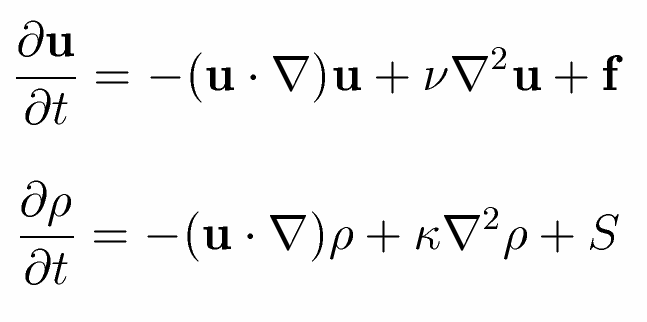
\includegraphics[width=5cm]{img/navierstokes.png}
    \caption{The Navier-Stokes Equations for the velocity in a compact vector notation (top) and the equation for a density moving through the velocity field (bottom).}
    \label{fig:navierstokes}
\end{figure}
We define a grid where both the density and velocity are defined at the cell centers. The grid contains an extra layer of cells to account for the boundary conditions.

\subsection{Density}
The paper of Stam \cite{stable} presents us with a solver for the velocity and density Navier-stokes equation at each time step. For the density equation there are three terms on the right hand side of the equation. The first term says that the density should follow the velocity field, the second states that the density may diffuse at a certain rate and the third term says that the density increases due to sources.\\
The fist step is solved by modeling the density as a set of particles. Start with two grids: one that contains the density values from the previous time step and one that will contain the new values. For each grid cell of the latter we trace the cell’s center position backwards through the velocity field. We then linearly interpolate from the grid of previous density values and assign this value to the current grid cell. The second step is solved by exchanging the density of each cell with its direct neighbors, as shown in Figure~\ref{fig:diffuse}.

\begin{figure}[h]
    \centering
    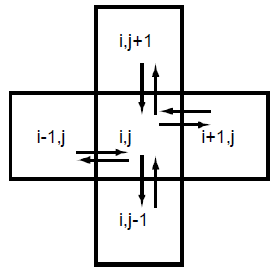
\includegraphics[width=4cm]{img/diffuse.png}
    \caption{Through diffusion each cell exchanges density with its direct neighbors.}
    \label{fig:diffuse}
\end{figure}

Adding density within a cell can be done when the users selects it with the mouse. Using diffusion and advection this source will automatically spread.


\subsection{Velocity}
The velocity field uses the same advection and diffusion step as the density field, but diffusion is defined by viscosity. This is because the Navier-Stokes Equations are very similar. The only extra addition to the velocity step is mass conservation. This is an important property of real fluids which should be enforced. Mass conservation is done, by solving a linear system involving the gradient of the velocity field as described in \cite{stable}.

\subsection{Boundry}
We assume that the fluid is contained in a box with solid walls: no flow should exit the walls. This simply means that the horizontal component of the velocity should be zero on the vertical walls, while the vertical component of the velocity should be zero on the horizontal walls. This is accomplished by inverting the velocity (w.r.t. x and y) on the boundaries and copying the density of its neighbours.

\section{Fixed Objects}
The user can add fixed objects by pressing the middle mouse button. Fixed objects are maintained using a grid, that has the same size as the velocity and density grids. If a cell contains a fixed objects the value is 1, otherwise the value is 0. Each component of fixed objects consists of 5 cells. The structure is as shown in Figure~\ref{fig:fixedstructure}.

\begin{figure}[h]
    \centering
    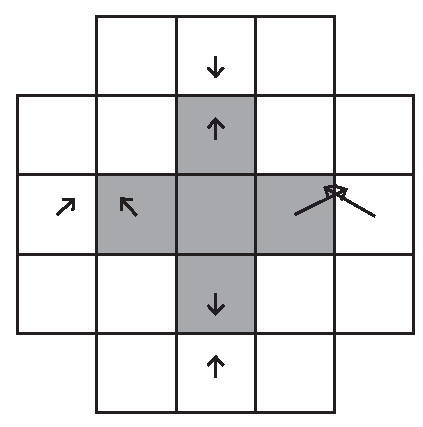
\includegraphics[width=5cm]{img/fixedstructure.pdf}
    \caption{Structure of fixed object, with boundary conditions examples for velocity.}
    \label{fig:fixedstructure}
\end{figure}

This structure is convenient because the velocity for each side can be calculated separately. For example, the velocity on the top of the fixed object only uses velocity of its top neighbour. So when a fluid is directed to the top of the fixed object, it will 'bounce' in the y-axis and remain its horizontal trajectory. The mechanism is the same as the boundary conditions, and is also calculated each time boundary conditions for the outer wall are calculated. Figure \ref{fig:fixed} shows the boundary conditions of the fixed objects. The fluid is trapped inside the square of fixed objects because it bounces back on the boundaries of the fixed objects.

\begin{figure}[H]
    \centering
    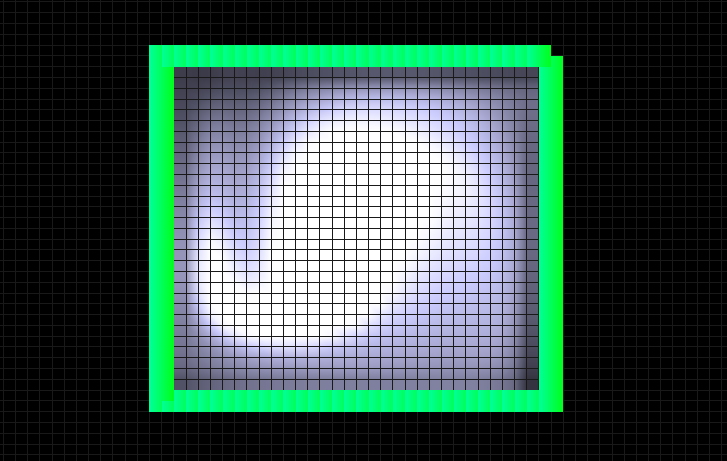
\includegraphics[width=8cm]{img/fixed.png}
    \caption{Fluid trapped inside a square of fixed objects.}
    \label{fig:fixed}
\end{figure}

\section{Particles and Fluids}
	Direct port of previous
	Pressure/Drag force
\section{Moving objects and Rigid Bodies}
Moving solid objects and rigid bodies are implemented using particles. The only difference between solid objects and rigid bodies is that rigid bodies can rotate and solid objects can not. Objects are defined by a polygon, where the points of the polygon are represented by particles. Forces acting on the particles are directly converted to the object. Furthermore, the center of mass of an object is defined by the location of the object. Lastly, next to the mass of the object, an object has a mass moment of inertia measuring the rigid's ability to resist changes in rotational speed.

\subsection{Boundry conditions}
To make the fluid act more naturally around the boundary of an object, also boundary conditions for objects are introduced. Boundary conditions for objects are defined the same way as boundary conditions for fixed objects. To find the cells of the fluid grid which are on the boundary of the object, we firstly find the bounding box of the object. Then we check for each cell in the bounding box if it contains a part of the boundary of the object or if the cell is completely inside the object.\\
Then for cells which contain a boundary, the same technique as boundary conditions for fixed objects is used. For cells which are inside an object, all components (velocity and density) are set to zero such that they do not have any influence on the object. The downside of setting the fluids density to zero within the object is that the object will remove most of the density, since the boundary force is not sufficient enough to push the fluids away, but it looks more realistic, because the objects leaves a trail as can be seen in figure \ref{fig:trail}.

\begin{figure}[!htb]
\centering
  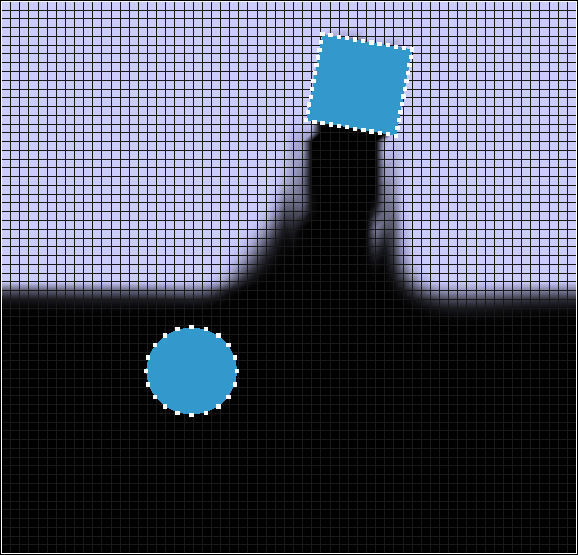
\includegraphics[height=0.5\textwidth]{img/trail}
  \captionof{figure}{Rigid body being dragged by a spring force through the fluid leaving a trail}
  \label{fig:trail}
\end{figure}

\subsection{Object forces}
The total force on an object is defined as $F = \sum{F_i}$, where $F_i$ is the force acting on particle $p_i$ and the total torque on a rigid body is $\tau = \sum{((r_i - x) \times F_i)}$, where $r_i$ is the world position of particle $p_i$. The mass moment of inertia of a body is dependant on the shape of the object. We implemented two type of objects, a rectangle and a disk. The mass moment of inertia $I$ for those object are $I_r =  m (w^2 + h^2)$ and $I_d = \frac{mr^2}{2}$ for a rectangle and a disk respectively.\\
There are two ways in which forces can be applied to an object. Firstly, the fluids pressure can apply forces to the particles of an object as described in the previous section. Secondly the user is able to select one of the particles of an object to create a spring force between the mouse cursor and the particle. Also to make sure an object comes to rest naturally, a drag force is used for both linear and angular velocity. In figure \ref{fig:fluidobject} it can be seen that the fluid exerts force on rigid bodies.
\begin{figure}[!htb]
\centering
  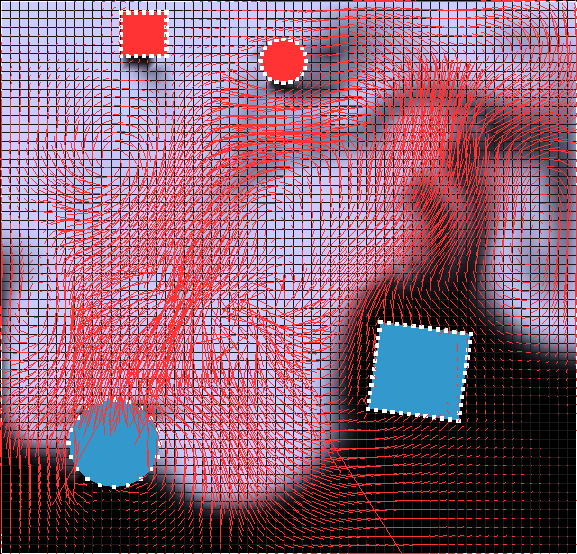
\includegraphics[height=0.5\textwidth]{img/fluidobject}
  \captionof{figure}{Rigid bodies being moved by forces exerted by the fluid}
  \label{fig:fluidobject}
\end{figure}
\subsection{Object to fluid coupling}
To make the simulation more realistic, solid objects and rigid bodies also exert forces to the fluids. This is done by adding velocity to the velocity field around the object. To find the cells around the object, just like with the boundary conditions, we find the bounding box of the object and then find the cells which contain a part of the boundary of the object. Then for the cells next to the boundary, we add a fraction of objects velocity to these cells, such that the density around the object will also be advected in the direction in which the object is moving. The influence of the object on the velocity field can be seen in figure \ref{fig:objectfluid}.

\begin{figure}[!htb]
\centering
  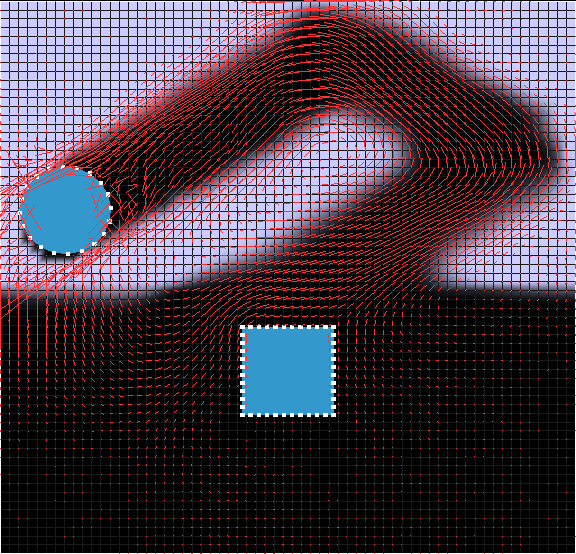
\includegraphics[height=0.5\textwidth]{img/objectfluid}
  \captionof{figure}{Moving rigid body influences velocity field}
  \label{fig:objectfluid}
\end{figure} 
\section{Results}
In the figures below some scenes are shown of the final result.

\begin{figure}[h!]
\centering
\begin{minipage}[t]{.40\textwidth}
  \centering
  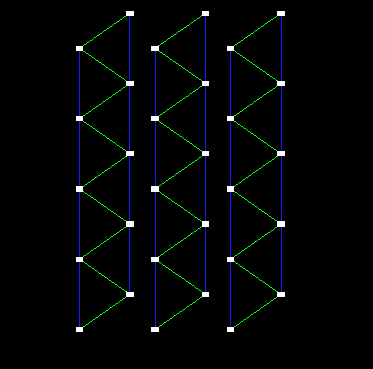
\includegraphics[height=5cm]{img/resulthair.png}
  \captionof{figure}{Start position of hair}
  \label{fig:hair}
\end{minipage}\hfill
\begin{minipage}[t]{.50\textwidth}
  \centering
  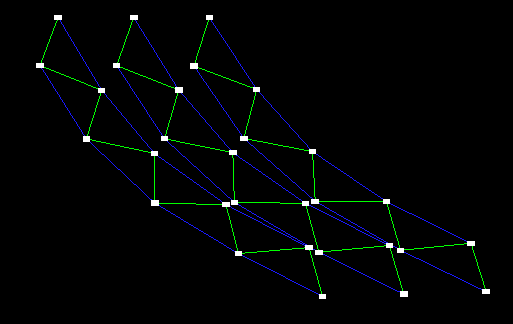
\includegraphics[height=5cm]{img/resulthair2.png}
  \captionof{figure}{Hair position after some iterations}
  \label{fig:hair2}
\end{minipage}
\end{figure}

\begin{figure}[h!]
\centering
\begin{minipage}[t]{.45\textwidth}
  \centering
  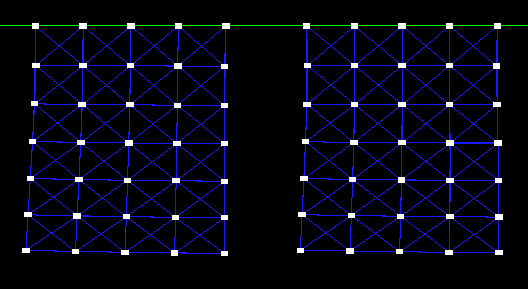
\includegraphics[height=4cm]{img/curtain.png}
  \captionof{figure}{Start position of two cloth curtains }
  \label{fig:flag}
\end{minipage}\hfill
\begin{minipage}[t]{.45\textwidth}
  \centering
  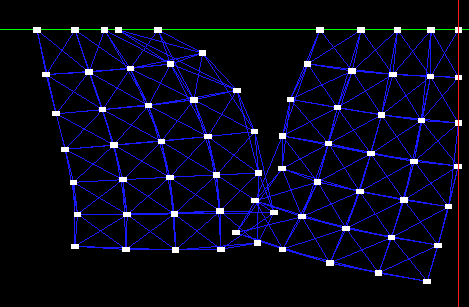
\includegraphics[height=4cm]{img/curtain2.png}
  \captionof{figure}{Two cloth curtains colliding}
  \label{fig:flag2}
\end{minipage}
\end{figure}




\section{Conclusion}

We started with the implementation of a global system to solve all forces and constraints.
With these forces and constraints we made some nice scenes such as hair and cloth, as shown in the results.
The user can also apply forces by interacting with the mouse.
Because the euler integration method is not very stable other integration methods where implemented.
Finally collision detection is implemented such as particle collisions and fixed object collisions.

\begin{thebibliography}{1}
\bibitem{stable}
    J. Stam,
    \emph{Real-Time Fluid Dynamics for Games},
    Toronto, Ontario, Canada.
\end{thebibliography}
    
\end{document}
